%File: main.tex
\documentclass[letterpaper]{article}
\usepackage{aaai}
\usepackage{times}
\usepackage{helvet}
\usepackage{courier}
\usepackage{graphicx}
\usepackage{amsmath}
% \usepackage{booktabs}
\frenchspacing
\setlength{\pdfpagewidth}{8.5in}
\setlength{\pdfpageheight}{11in}
\pdfinfo{
/Title (Baewatch:\\regola di voto per un sistema di raccomandazione di gruppo)
/Author (Alessandro Pasqualini)}
\setcounter{secnumdepth}{0}  
\begin{document}
% The file aaai.sty is the style file for AAAI Press 
% proceedings, working notes, and technical reports.
%
\title{Baewatch:\\regola di voto per un sistema di raccomandazione di gruppo}
\author{Alessandro Pasqualini\\
Dipartimento di Ingegneria dell'Informazione\\
Università di Padova, Padova\\
alessandro.pasqualini@studenti.unipd.it\\
}
\maketitle
\begin{abstract}
\begin{quote}
Al giorno d'oggi i sistemi di raccomandazione veicolano le scelte degli utenti in moltissimi settori, accumulando conoscenza sulle loro preferenze. Queste preferenze sono successivamente elaborate da specifici algoritmi per predire e consigliare all'utente il suo nuovo acquisto, il prossimo film da vedere, etc. Le informazioni ottenute sono incrociate con quelle di altri utenti migliorandone l'accuratezza.

Una delle sfide più importanti è quella di utilizzare le preferenze dei vari utenti per ottenere delle raccomandazioni di gruppo, dove si rivela necessario soddisfare interessi differenti e a volte contrastanti tra di loro. In questo contento nasce Baewatch, una regola di voto il cui scopo è selezionare una raccomandazione per il gruppo in modo da massimizzare la "contentezza" di ogni componente.

\end{quote}
\end{abstract}

\section{Introduzione}
Internet ha assunto negli anni un ruolo sempre più centrale nella vita quotidiana, arrivando a diventare uno dei principali mercati dove poter acquistare un numero sempre maggiore di beni. Il numero esponenziale di possibilità di acquisto ha spinto lo sviluppo e la realizzazione di sistemi di raccomandazione in modo da consigliare ed indirizzare l'utente nella scelta.

All'interno di alcuni settori, ad esempio lo streaming di film e serie tv, questi sistemi si sono rivelati essenziali per il successo di alcuni dei principali player. Netflix, Amazon, Google devono parte del loro successo commerciale a questi algoritmi, al punto di diventare parte essenziale della loro offerta.

\begin{figure}[!htb]
    \begin{centering}
        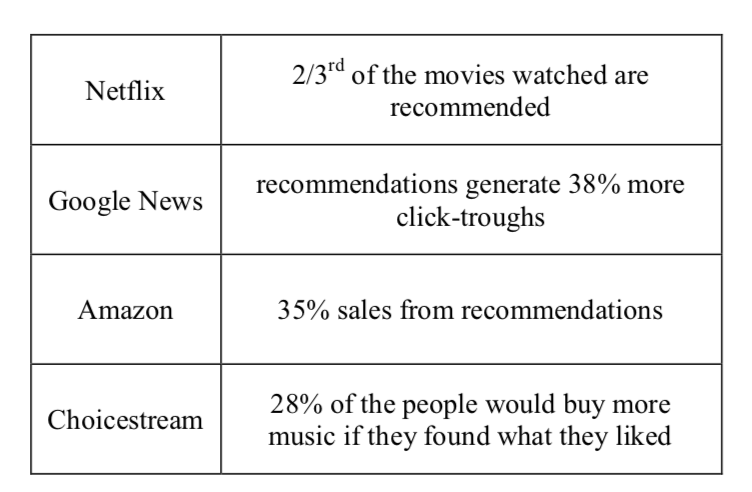
\includegraphics[width=\linewidth]{Figures/successo.png}
        \caption{Successo dei sistemi di raccomandazione di alcune piattaforme \cite{ref1}}
        \label{fig:successo}
    \end{centering}
\end{figure}

Le raccomandazioni fornite dai sistemi di raccomandazioni possono essere accettate oppure ignorate da parte dell'utente. Le interazioni, dirette o indirette, che l'utente ha nei confronti di quanto consigliato dal sistema compogono un insieme di informazioni che vengono utilizzate dallo stesso sistema per migliorare la sua qualità in futuro.

Questi sistemi possono sfruttare modelli, quali il collaborative filtering, in modo da incrociare le informazioni di altri utenti ritenuti simili, secondo qualche metrica, per assegnare un rating ad un bene non ancora valutato dall'utente.

Una delle principali sfide dei sistemi di raccomandazione è fornire delle raccomandazioni per gruppi di utenti, bilanciando bisogni e scelte differenti dei vari membri. Un esempio può essere proprio la raccomandazione di un film ad un gruppo di persone: in questo contesto è possibile riconoscere alcune difficoltà non presenti nel contesto individuale. Alcuni membri del gruppo potrebbero avere interessi competitivi e pertanto sarà l'intero gruppo ad accettare o rifiutare la proposta generata.

\section{Collaborative Filtering}
Un sistema di raccomandazione è un sistema che, attraverso tecniche di filtraggi delle informazioni, cerca di raccomandare all'utente degli oggetti che possano essere di suo interesse \cite{ref2}. 

In un contesto individuale, più l'utente interagisce con il sistema, accettando o rifiutando le raccomandazioni, più il sistema può migliorare le sue predizioni, fornendo raccomandazioni via via sempre più accurate. All'interno del sistema convivono più utenti e tutti questi utenti, in un modo o nell'altro, chi più chi meno, interagiscono con il sistema di raccomandazioni che si trova quindi nella posizione privilegiata di raccogliere moltissime informazioni sulle preferenze degli utenti. In questo contesto nasce il \emph{Collaborative Filtering}, un sistema che utilizza le informazioni degli altri utenti per determinare delle raccomandazioni per un determinato utente.

Le informazioni che il collaborative filtering usa sono principalmente i rating assegnati agli oggetti da parte degli utenti del sistema. \`E possibile distinguere due modalità, anche se non sono le uniche, che permettono di aggregare questi rating per ottenere una stima per un utente su un oggetto non ancora preso in considerazione e che sarà quindi il risultato della raccomandazione.

La prima modalità è chiamata \emph{user based}: il sistema determina, secondo alcune metriche, degli utenti che assomigliano a quello destinatario della raccomandazione e sfrutta i rating di questi utenti per stimare una valutazione dell'oggetto da raccomandare. Algoritmi molto usati per questo determinare il grado di somiglianza tra gli utenti sono il \emph{cosine similarity} o il \emph{pearson correlation}. La stima del rating è ottenuta eseguendo una media pesata (secondo coefficienti dipendenti dall'algoritmo) dei singoli rating assegnati dagli utenti.

Un'altra possibilità è l'utilizzo di collaborative filtering \emph{item based}. In questo caso caso viene determinata una similarità tra oggetti e non più tra utenti: per stimare il voto dell'utente destinatario della raccomandazione si usano comunque i rating degli utenti attribuiti a quell'oggetto. Il collaborative filtering item based, chiamato anche item-item per enfatizzare il ruolo primario degli oggetti rispetto agli utenti, è stato inventato da Amazon per rispondere ad alcune problematiche dall'altra modalità: performance non ottimali nel caso di grossa disparità tra il numero di oggetti e il numero di utenti, dove il primo è di parecchio più grande del secondo. \`E chiaro che se il numero degli utenti è molto inferiore al numero degli oggetti allora risulta difficile trovare utenti simili a quello per cui la raccomandazione viene generata e di conseguenza la qualità stessa della raccomandazione ne risente pesantemente.

Il collaborative filtering è dunque usato per sistemi di raccomandazione individuali e non di gruppo. Nei sistemi di gruppo si pongono difficoltà differenti, tra le quali è possibile evidenziare la difficoltà di aggregazione dei voti stimati per i singoli utenti dovendo bilanciare diversi interessi che è bene ricordare, possono essere contrastanti tra di loro. 

In questo progetto si è cercato di fornire una regola di voto per determinare una raccomandazione di un film ad un gruppo di persone. Nel contesto proposto come esempio è ragionevole supporre che la raccomandazione consista im un lungometraggio non visto da nessuno dei membri del gruppo. Per questo motivo il primo stadio è l'utilizzo del collaborative filtering user based per stimare il rating dei vari componenti sul sottoinsieme dei film presenti a catalogo non ancora visionati.

\section{La regola di voto Baewatch}
L'ambito evidenziato della raccomandazione di un film per un gruppo di persone può essere rappresentato come un contesto multi agente avversario: tutti gli utenti forniscono un rating per ogni elemento, seppur stimato dal primo stadio di collaborative filtering. Ogni utente compete quindi con gli altri per raccomandare la sua \emph{top choice} a tutto il gruppo. La regola di voto è quindi chiamata ad eseguire un trade off per massimizzare il grado di "contentezza" di tutto il gruppo e non solo di un componente.

\`E bene anche porre l'attenzione sul fatto che la top choice di un utente non corrisponde automaticamente all'elemento con rating 5, ovvero il massimo possibile dei rating (i voti sono disposti su una forbice da 1 a 5), ma è molto più plausibile che sia un valore inferiore. Un elemento è considerato top choice di un utente se gli è stato assegnato il punteggio più elevato rispetto agli altri elementi valutati per conto dell'utente (il rating è fornito dallo stadio di collaborative filtering e non direttamente dall'utente). Allo stesso modo siamo in presenza di un ordinamento parziale e quindi è possibile che un utente possegga più top choice. Non verrà fatta differenza tra una top choice e l'altra, nel caso in cui siano multiple, entrambe concorrono ugualmente alla determinazione della raccomandazione di gruppo.

L'idea che sta alla base della regola di voto \emph{Baewatch} è quella di massimizzare la "contentezza" dell'\emph{intero} gruppo, definendo una metrica di costo. La regola \emph{Baewatch} propone di assegnare un costo ad ogni tupla di voti dei vari utenti allo stesso elemento, lo stesso film nel contesto analizzato. Questo costo è frutto di una metrica il cui scopo è massimizzare la "contentezza" dell'\emph{intero} gruppo, scegliendo la tupla più distante dal valore minino di rating, ovvero la tupla con voti tutti pari a 1.

La metrica di costo, come evidenziato, assegna un costo \emph{non lineare} ai vari rating stimati per conto dell'utente. Il costo della tupla è la somma di questi costi singoli.

\begin{equation}
    r_{i,j} = (R - u_{i,j})^2
\end{equation}

dove $R$ rappresenta il rating massimo assegnabile, 5 in questo contesto, $u_{i,j}$ è il rating stimato per l'utente $i$ per l'elemento $j$ da parte dello stadio di collaborative filtering ed infine $r_{i,j}$ è il costo del rating per questo utente. Per ottenere il rating $r_{j}$ dell'intera tupla basta sommare i singoli rating degli utenti.

\begin{equation}
    r_j = \sum_{i=1}^{N} r_{i,j} = \sum_{i=1}^{N} (R - u_{i,j})^2
\end{equation}

Analizzando il costo ottenuto per ogni utente, $r_{i,j}$, vediamo come sia non lineare, ovvero è il quadrato della differenza tra il voto massimo e il voto stimato per l'utente. Questa scelta fa sì che il costo sia tanto maggiore tanto il rating è vicino a 1. Nell'estremo opposto abbiamo, quando il rating dell'utente è 5, l'annullamento del costo e questo è dovuto al fatto che l'elemento corrente è la top choice dell'utente. La regola di voto è quindi aurotizzata ad effettuare un trade off cercando di massimizzare il rating minimo assegnato da un utente a spese degli altri componenti del gruppo. Naturalmente non può penalizzare eccessivamente gli utenti con rating alto in quando la dipendenza quadratica fa sì che ad un certo punto il costo diventi eccessivo e quindi la tupla venga scartata.

Per ottenere la raccomandazione, una volta ottenuto $r_{j}$ per ogni elemento è sufficiente ordinare per costi crescenti e selezionare il primo elemento di questa lista ordinata. \`E chiaro che per le premesse effettuate sopra, si è in presenza di un ordinamento parziale ed è quindi possibile che l'algoritmo assegni costo minimo a più tuple: è sufficiente restituire una delle soluzioni.

Per chiarire il funzionamento è utile un esempio.

\begin{table}[h]
\centering
\begin{tabular}{|l|c|c|}
\hline
\textbf{User} & \multicolumn{1}{l|}{\textbf{Item1}} & \multicolumn{1}{l|}{\textbf{Item2}} \\ \hline
User1         & 4                                   & 4                                   \\ \hline
User2         & 3                                   & 4                                   \\ \hline
User3         & 5                                   & 4                                   \\ \hline
User4         & 2                                   & 2                                   \\ \hline
\end{tabular}
\caption{Voti assegnati dagli utenti a due oggetti}
\label{table:1}
\end{table}

Nella Tabella \ref{table:1} vediamo i voti stimati da parte del collaborative filtering per quattro utenti su due oggetti. A questo punto è possibile calcolare il costo assegnato da \emph{Baewatch} alle due tuple.

\begin{equation}
    r_1 = (5 - 4)^2 + (5 - 3)^2 + (5 - 5)^2 + (5 - 2) ^2 = 14
\end{equation}
\begin{equation}
    r_2 = (5 - 4)^2 + (5 - 4)^2 + (5 - 4)^2 + (5 - 2) ^2 = 12
\end{equation}

Quindi la tupla migliore risulta essere la seconda, ovvero quella con \emph{Baewatch cost} minore tra le due.        

\section{Esempi di applicazione di Baewatch}
Per concludere la trattazione della regola di voto Baewatch è interessante studiarne l'applicazione su alcuni casi di interesse. Si suppone che che i voti siano frutto del primo stadio di collaborative filtering non riportato.

\begin{table}[h]
\centering
\begin{tabular}{|l|c|c|}
\hline
\textbf{User}          & \multicolumn{1}{l|}{\textbf{Item1}} & \multicolumn{1}{l|}{\textbf{Item2}} \\ \hline
User1                  & 5                                   & 5                                   \\ \hline
User2                  & 5                                   & 5                                   \\ \hline
User3                  & 5                                   & 5                                   \\ \hline
User4                  & 1                                   & 2                                   \\ \hline
\textit{Baewatch cost} & \textit{16}                         & \textit{9}                          \\ \hline
\end{tabular}
\caption{Applicazione di Baewatch ad rating differenti solo per un voto}
\label{table:2}
\end{table}

Nella Tabella \ref{table:2} sono riportati i voti dati da alcuni utenti a due oggetti, \emph{item1} e \emph{item2}. Queste due tuple di voti differiscono solamente per il rating assegnato dall'utente \emph{User4} ai due oggetti: nel primo caso ha attribuito il voto 1 mentre nel secondo il voto 2. Il cambiamento del valore \emph{Baewatch cost} è quindi imputabile solamente a utente \emph{User4} e questo modifica la scelta finale dell'algoritmo dalla prima tupla alla seconda. L'algoritmo preferisce dunque la seconda tupla in quanto presenta un costo inferiore, in linea con il principio di scegliere la tupla "più distante" dal rating minimo.

\begin{table}[h]
\centering
\begin{tabular}{|l|c|c|c|c|}
\hline
\textbf{User}          & \multicolumn{1}{l|}{\textbf{Item1}} & \multicolumn{1}{l|}{\textbf{Item2}} & \multicolumn{1}{l|}{\textbf{Item3}} & \multicolumn{1}{l|}{\textbf{Item4}} \\ \hline
User1                  & 5                                   & 5                                   & 4                                   & 1                                   \\ \hline
User2                  & 5                                   & 5                                   & 4                                   & 1                                   \\ \hline
User3                  & 5                                   & 5                                   & 4                                   & 1                                   \\ \hline
User4                  & 1                                   & 2                                   & 5                                   & 1                                   \\ \hline
\textit{Baewatch cost} & \textit{16}                         & \textit{9}                          & \textit{3}                          & \textit{64}                         \\ \hline
\textit{Mean}          & \textit{4}                          & \textit{4,25}                       & \textit{4,25}                       & \textit{1}                          \\ \hline
\textit{Var}           & \textit{3}                          & \textit{2,31}                       & \textit{0,15}                       & \textit{0}                          \\ \hline
\end{tabular}
\caption{Confronto del \textit{Baewatch cost} con \textit{media} e \textit{varianza}}
\label{table:3}
\end{table}

\`E naturale a questo punto proporre un confronto tra la metrica di costo proposta, alla base della regola di voto Baewatch, con media e varianza delle tuple. In Tabella \ref{table:3} sono riportati dei rating di quattro utenti (eventualmente ottenuti attraverso il primo stadio di collaborative filtering) assegnati a due oggetti. Nella tabella sono riportati anche Baewatch cost, media e varianza delle tuple. La quarta tupla è quella che possiede il rating peggiore, tutti gli utenti hanno assegnato il valore minimo; d'altra parte però anche la varianza è minore, indicando che i membri del gruppo sono concordi nella votazione. La varianza effettivamente può essere intesa come una "misura" di quanto i membri del gruppo siano concordi nella votazione. Baewatch ha però come obiettivo massimizzare la "contentezza" del gruppo e non il loro grado di "concordanza". Analizzando sotto questa luce è possibile comprendere allora il perchè del costo maggiore assegnato all quarta tupla: è quella peggiore ottenibile con i voti di quattro utenti espressi nell'intervallo 1-5 e qualsiasi altra tupla sarà sicuramente migliore. La quarta tupla rappresenta effettivamente il punto da cui Baewatch cerca di "allontanarsi".


\begin{table}[h]
\centering
\begin{tabular}{|l|c|c|}
\hline
\textbf{User}          & \multicolumn{1}{l|}{\textbf{Item1}} & \multicolumn{1}{l|}{\textbf{Item2}} \\ \hline
User1                  & 4                                   & 5                                   \\ \hline
User2                  & 4                                   & 5                                   \\ \hline
User3                  & 4                                   & 5                                   \\ \hline
User4                  & 2                                   & 1                                   \\ \hline
\textit{Baewatch cost} & \textit{12}                         & \textit{16}                         \\ \hline
\textit{Mean}          & \textit{3,5}                        & \textit{4}                          \\ \hline
\textit{Var}           & \textit{0,75}                       & \textit{3}                          \\ \hline
\end{tabular}
\caption{Baewatch massimizza la "contentezza" del gruppo e non dei singoli componenti}
\label{table:4}
\end{table}

L'ultimo esempio proposto, riportato in Tabella \ref{table:4} è anche quello probabilmente più interessante. \`E possibile infatti notare come la regola di voto assegni un costo minore alla prima tupla anche se la seconda ha media superiore. Questo fatto è spiegabile considerando che il principio della regola di voto \emph{Baewatch} è quello di aumentare il grado di "contentezza" dell'\emph{intero} gruppo e non quello dei singoli componenti. L'algoritmo è quindi "disposto" a penalizzare leggermente i primi tre utenti, che comunque mantengono un rating di 4 su 5, per aumentare di uno il voto del quarto membro. Questo comportamento rispecchia quello evidenziabile nella vita reale: la scelta spesso ricade su una soluzione non ottima, ma comunque non molto lontana da essa per alcuni componenti, per favorire quei pochi membri che in caso contrario otterrebbero la soluzione per loro peggiore.

\section{Conclusioni}
Baewatch è una regola di voto che permette di eseguire delle scelte su tuple di voti degli utenti in modo da massimizzare il livello di "contentezza" dell'intero gruppo. Le prestazioni dell'intero sistema dipendono in maniera elevata da quelle dello stadio di Collaborative Filtering, dove vengono fornite delle possibili stime che gli utenti potrebbero assegnare ad elementi che non hanno ancora mai preso in considerazione. \`E chiaro che se la qualità dei rating di questo stadio è bassa la scelta eseguita da Baewatch difficilmente verrà accettata dal gruppo, il quale sarà chiamato a valle della scelta ad esprimere l'accettazione o meno di quanto proposto.

Baewatch è una regola di voto deterministica e di conseguenza in caso di rifiuto della raccomandazione da parte dell'intero gruppo è evidente come la causa sia principalmente da attribuire allo stadio iniziale di Collaborative Filtering. D'altra parte Baewatch è lontano dal poter essere ritenuto un algoritmo ottimale in quando si basa sull'idea non totalmente definita di "contentezza di un gruppo". Questo concetto è difficilmente esprimibile in termini matematici perché gli stessi membri potrebbero avere degli interessi competitivi: basti pensare ad un gruppo formato da persone dove ogni componente preferisce un genere di film totalmente differente. In questo contesto risulta difficile bilanciare gli interessi e determinare il lungometraggio che possa incontrare l'interesse di tutti i membri del gruppo, anche se effettivamente un film difficilmente può essere inquadrato in una singola categoria. Baewatch si trova quindi a dover intraprendere un gran numero di trade off tra le varie tuple di voti per ottenere una raccomandazione da proporre all'intero gruppo.

D'altra parte i test effettuati sul dataset MovieLens (https://grouplens.org/datasets/movielens/100k/) e sugli esempi proposti nel precedente paragrafo evidenziano le potenzialità di questa regola in contesti di raccomandazione di gruppo. Sicuramente è possibile migliorare la metrica di costo tenendo in considerazione anche media e varianza dei voti delle tuple, magari determinando dei coefficienti per pesare queste tre componenti che giocano un ruolo centrale in questo tipo di raccomandazioni.

\section{Materiale aggiuntivo}
Una prima implementazione in Pyhton dell'algoritmo presentato è disponibile presso https://github.com/alessandro1105/baewatch. All'interno del repository è possibile trovare il file \emph{test\_complete.py} che permette di valutare l'algoritmo utilizzando il MovieLens 100K Dataset (https://grouplens.org/datasets/movielens/100k/). Il file \emph{test\_paper.py} contiene i test cases presentati in questo documento, insieme ad altri non citati, per dimostrare l'efficacia della regola di voto.

\bigskip

\bibliographystyle{aaai} 
\bibliography{bibliography}

\end{document}